\chapter{Rowerowe układy napędowe}

%______________________________________________________________________________________________________________
\section{Przekładnie mechaniczne}
Układ napędowy to zestaw urządzeń wykorzystywany do napędzania, w skład którego wchodzi źródło energii, układy pośredniczące w przekazywaniu energii oraz odbiornik energii. Mianem napędu zazwyczaj określa się urządzenia pośredniczące. Najczęściej wykorzystywanymi źródłami energii są silniki, a odbiorniki energii, których zadaniem jest realizowanie odpowiednich ruchów roboczych, przyjmują różne formy zależne od aplikacji.

Układ mechaniczny wykorzystany do przeniesienia ruchu obrotowego z elementu czynnego na element bierny nazywany jest przekładnią mechaniczną. Element czynny to element napędzający, natomiast element bierny to element napędzany. Oprócz transmisji energii, przekładnie umożliwiają również zmianę parametrów ruchu - momentu obrotowego oraz prędkości obrotowej. Przekładnie mechaniczne dzieli się na trzy grupy: cięgnowe, cierne i zębate. Przekładnie cięgnowe, które zostały opisane ze względu na zastosowanie w rowerowych układach napędowych, składają się z co najmniej dwóch kół, rozsuniętych względem siebie, oraz cięgna opasającego. Ze względu na rodzaj zastosowanego cięgna, wyróżnia się przekładnie pasowe oraz łańcuchowe. Przenoszenie mocy oraz momentu obrotowego jest możliwe dzięki występującym siłą tarcia pomiędzy kołem a cięgnem(połączenia cierne), lub poprzez zazębianie się koła z cięgnem(połączenia kształtowe).
\begin{figure}[h]
    \centering
    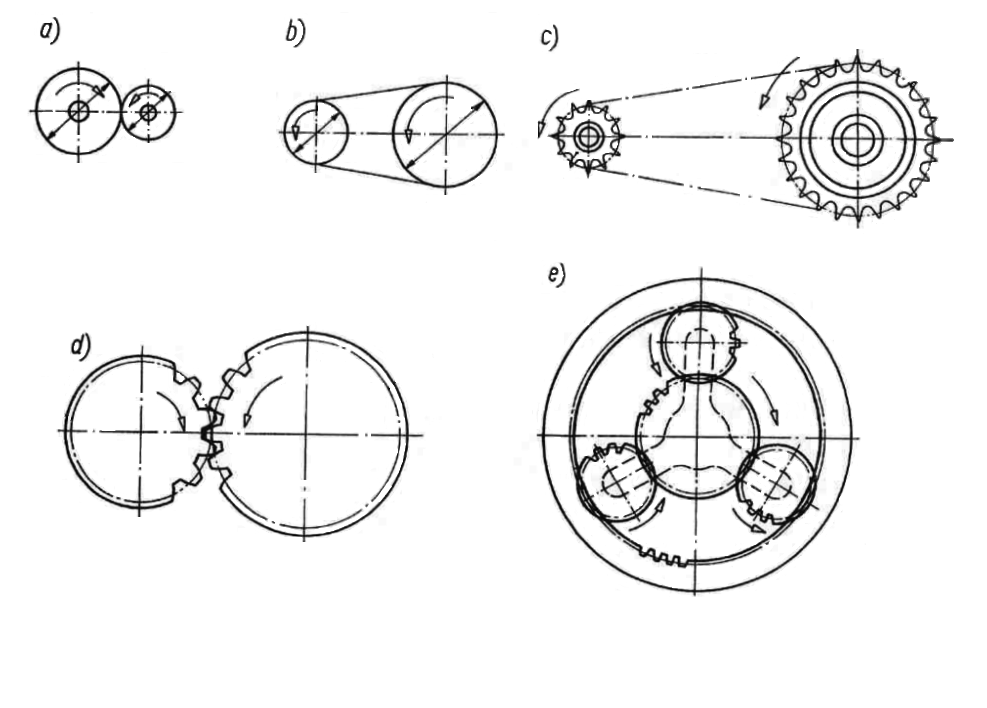
\includegraphics[scale=0.4]{przekladnie.png}
    \caption{Różne rodzaje przekładni mechanicznych: a) przekładnia cierna, b) przekładnia cięgnowa pasowa, c) przekładnia cięgnowa łańcuchowa, d - e) przekładnie zębate. Grafika opracowana na podstawie \cite{maszyny1}.}
    \label{fig:przekladnia}
\end{figure}

Wielkością charakteryzującą przekładnie jest przełożenie. Wyróżnia się przełożenie geometryczne, kinematyczne oraz dynamiczne. Przełożenie kinematyczne to stosunek prędkości kątowej koła czynnego do prędkości kątowej koła biernego\cite{przekladnie}:
\begin{equation}
    i = \frac{\omega_1}{\omega_2}
    \label{eq:przelozenieKinematyczne}
\end{equation}
\begin{eqwhere}[2cm]
	\item[$\omega_1$] prędkość kątowa koła czynnego
	\item[$\omega_2$] prędkość kątowa koła biernego
\end{eqwhere}

Przełożenie przekładni jest parametrem bezwymiarowym. Ze względu na wartość przełożenia przekładni wyróżnia się:
\begin{itemize}
\item
Przekładnie przyspieszające lub tzw. multiplikatory. Przekładnie tego typu zwiększają prędkość kątową koła biernego względem prędkości kątowej koła czynnego przy jednoczesnym zmniejszeniu momentu obrotowego koła biernego względem momentu obrotowego koła czynnego. Przełożenie takiej przekładni jest liczbą z zakresu od 0 do 1.
\item
Przekładnie redukujące lub tzw. reduktory. Przekładnie tego typu działają w sposób odwrotny do przekładni przyspieszających - zmniejszają prędkość kątową koła biernego względem prędkości kątowej koła czynnego oraz zwiększają moment obrotowy koła biernego względem momentu obrotowego koła czynnego. Przełożenie przekładni redukującej jest zawsze większe od 1.
\end{itemize} 
%____________________________________________________________________________________________________________  
\section{Układ napędowy w rowerze}
W przypadku konwencjonalnego układu napędowego stosowanego w rowerach elementem napędzającym jest rowerzysta. Siła przyłożona do ramienia korby generuje moment obrotowy, który przenoszony jest, przy pomocy mechanizmu korbowego i łańcucha, na koło zębate przymocowane na stałe do piasty tylnego koła. Moment obrotowy koła napędzającego powoduje powstanie sił obwodowych, składających się na siłę napędową, która wprawia rower w ruch postępowy.

Układ napędowy roweru wykorzystanego w pracy składa się z mechanizmu korbowego z jednym kołem zębatym, łańcucha, kasety ośmiorzędowej oraz przerzutki tylnej. Koło zębate zamontowane w mechanizmie korbowym ma 34 zęby. Kaseta składa się z ośmiu kół zębatych, których liczba zębów należy do zakresu od 11 do 32. Przekładnia zastosowana w rowerze, niezależnie od aktualnego biegu, ma zawsze charakter multiplikatora.

Przerzutka tylna umożliwia zmianę przełożenia układu napędowego. Działa na zasadzie czworoboku przegubowego. Składa się z czterech członów połączonych przegubowo, tworzących zamknięty łańcuch kinematyczny. Pozycja wózka przerzutki, przymocowanego do jednego z członów, (Rys.\ref{fig:przerzutka}) utrzymywana jest dzięki zastosowaniu sprężyny napinającej oraz cięgna, połączonego z mechanizmem do zmiany przełożeń, zamontowanym w manetce. Dodatkowo przerzutka posiada mechanizm napinający łańcuch, tak aby zachować jego odpowiedni zwis, gwarantujący pełną funkcjonalność układu napędowego, niezależnie od aktualnej pozycji wózka przerzutki. 
\begin{figure}[h]
    \centering
    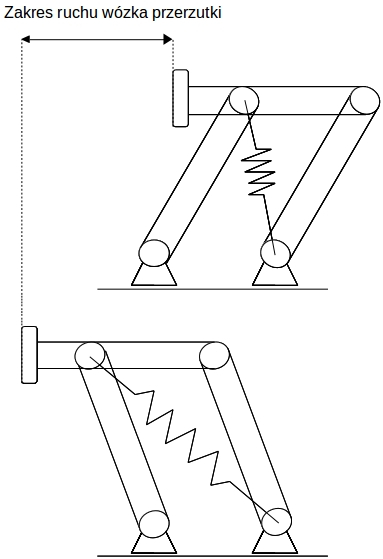
\includegraphics[scale=0.4]{przerzutka.jpg}
    \caption{Schemat ilustrujący zasadę działania konwencjonalnej tylnej przerzutki rowerowej.}
    \label{fig:przerzutka}
\end{figure}

\section{Układy napędowe oferowane na rynku komercyjnym}

Rosnące zainteresowanie branżą rowerową skutkuje wprowadzaniem na rynek coraz bardziej zaawansowanych technologicznie produktów. Dotyczy to właściwie każdego rodzaju części składających się na wyposażenie roweru. W momencie realizacji niniejszego projektu oferowanych na rynku jest co najmniej kilkanaście różnych rodzajów układów napędowych. Różnią się m.in. przeznaczeniem, ilością oferowanych przełożeń, zastosowanymi materiałami czy sposobem zmiany przełożeń.

Najbardziej ogólna klasyfikacja rowerowych układów napędowych to przeznaczenie. Można wyróżnić trzy główne grupy - kolarstwo szosowe, górskie oraz produkty przeznaczone do rowerów miejskich.

Kolarstwo szosowe stanowi główną siłę napędową rozwoju rowerowych układów napędowych. Coraz większe wymagania, pochodzące głównie z 
 
Napędy montowane w rowerach miejskich powinny charakteryzować się dużą niezawodnością, niską ceną oraz prostotą obsługi. Dodatkowo ważne jest, aby takie napędy były w miarę możliwości bezobsługowe. Sposób oraz charakter pokonywanych tras sprawia, że użytkownicy nie wymagają dużego zakresu przełożeń. Producenci sprzętu rowerowego nie rozwijają tej grupy napędów tak szybko, jak produktów przeznaczonych do zastosowania w kolarstwie górskim czy szosowym. Jedynym rozwiązaniem, na które według Autora warto zwrócić uwagę, są piasty wielobiegowe. Zmiana przełożenia jest możliwa dzięki zastosowaniu przekładni planetarnej, zamontowanej wewnątrz piasty tylego koła. Główne zalety tego rozwiązania to wysoki stopień integracji części mechanicznych ukrytych w piaście, brak konieczności przeprowadzania czynności serwisowych oraz prosta obsługa. Główni producenci rowerowych układów napędowych, a są to Shimano i SRAM, oferują kilka grup napędów tego rodzaju. Shimano posiada w swojej ofercie grupę Alfine oraz Nexus. SRAM oferuje produkty i-MOTION 3, Automatix oraz G8. 

   

